\documentclass[main]{subfiles}

\begin{document}
\section{Diskussion}
\subsection{Optimering af dataopsamling}
Resultaterne bærer præg af, at det er første gang vi arbejdede med et rigtigt laser setup. Målingerne tog lang tid, som et resultat af at udstyret er meget fintfølsom og at der var mange sikkerhedsmæssige hensyn at tage ift. laseren. Forsøgsopstillingen var nogenlunde optimeret, men små ændringer viste store virkninger på parametrene, hvorfor det er oplagt at nævne mange systematiske fejl.
\\
I modul et lader vi afstanden til skærmen være $l = \SI{29,8}{\centi\meter}$. En større afstand, ville resultere i at afstanden mellem laser-prikkene blev størrer hvorfor måleredskabets usikkerheder ville have mindre indflydelse. Derfor kunne forsøgets præcision optimeres. Ud over det kunne der med fordel være opsat millimeter-papir på skærmen, for at kunne måle afstanden mere præcist.
\\
I modul to kunne man have taget flere målinger for at minimere usikkerheder på det endelige resultat. Ydermere kunne man have brugt flere forskellige linser med forskellige fokallængder, idet at dette ville ændre på laserstrålens waist.
Hvis tiden tillod det kunne man også have kigget nærmere på forsøgsopstillingen, efter opstillingsfejl ved de målinger som gav meget store risetimes, idet at det sandsynligvis skyldes en fejl i opstillingen.
\begin{figure}
  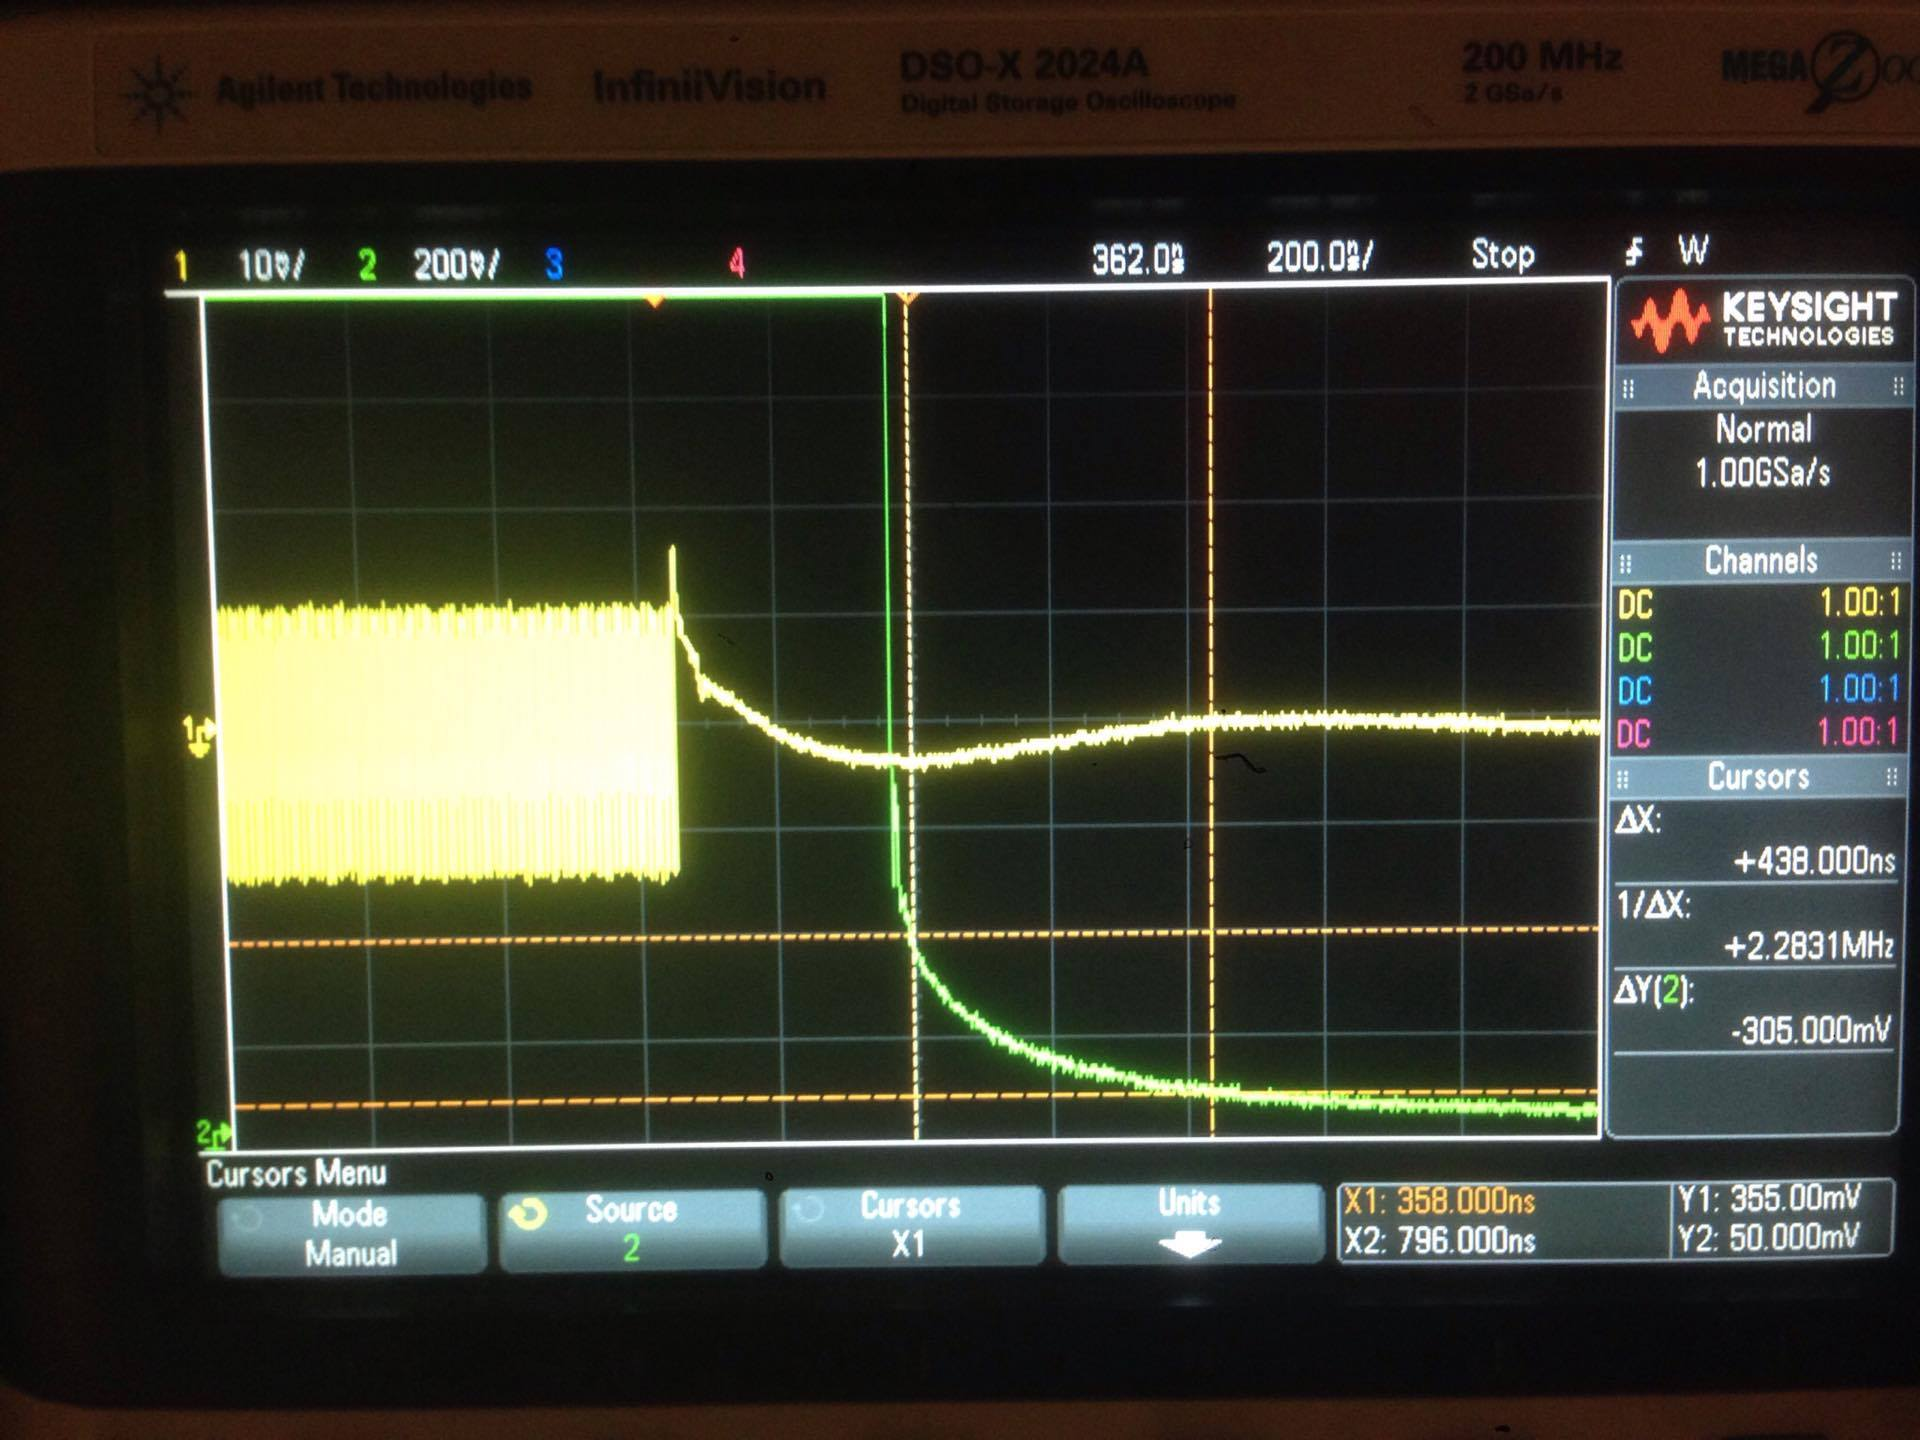
\includegraphics[width=\linewidth]{tegninger/BILAG.png}
  \caption{oscilloskopets display indstillet til at vise risetime som $\Delta x$}
  \label{BILAG}
\end{figure}
På \cref{BILAG} ses en sådan måling. Bemærk den høje risetime.
\subsection{Usikkerheder og fejlkilder}
Forsøget er afhængig af flere ukendte paremetre fra apparature som påvirker målingerne. Usikkerheden fra frekvensgeneratoren kendes ikke, men antages at være negligibel lille. Det anvendte powermeter svingede omkring en værdi, hvor usikkerheden af apparaturet skønnes til at være dette udsving. Endelig var der parametre, hvor usikkerheden ikke vides. $T_r$ var svær at vurdere, da usikkerheden både afhang af usikkerheden af placeringen af oscilloskopets cursor modes samt førnævnte oscilloskop.
\\
I forsøget lavede vi direkte fejl. Vi var uopmærksomme på at parameteren $I_0$ fra ligning \cref{eq:Intensitet} skulle noteres. Og dermed haves for mange ukendte til at kunne plotte over det ønskede. Dernæst, da vi skulle måle waist ved hjælp at føre kniven hele vejen igennem laserstrålen (\cref{fig:graf3}), placerede vi ikke kniven i hvad der formodes til at være fokalpunktet for linsen, så vores vi kunne ikke finde waist ved at fitte til \cref{eq:errorfunc}.



\end{document}
